%
%Не забыть:
%--------------------------------------
%Вставить колонтитулы, поменять название на титульнике



%--------------------------------------

\documentclass[a4paper, 12pt]{article} 

%--------------------------------------
%Russian-specific packages
%--------------------------------------
%\usepackage[warn]{mathtext}
\usepackage{cmap}					% поиск в PDF
\usepackage[T2A]{fontenc}
\usepackage[utf8]{inputenc}
\usepackage[english,russian]{babel}
\usepackage[intlimits]{amsmath}
\usepackage{esint}
%--------------------------------------
%Hyphenation rules
%--------------------------------------
\usepackage{hyphenat}
\hyphenation{ма-те-ма-ти-ка вос-ста-нав-ли-вать}
%--------------------------------------
%Packages
%--------------------------------------
\usepackage{amsmath}
\usepackage{amssymb}
\usepackage{amsfonts}
\usepackage{amsthm}
\usepackage{latexsym}
\usepackage{mathtools}
\usepackage{etoolbox}%Булевые операторы
\usepackage{extsizes}%Выставление произвольного шрифта в \documentclass
\usepackage{geometry}%Разметка листа
\usepackage{indentfirst}
\usepackage{wrapfig}%Создание обтекаемых текстом объектов
\usepackage{fancyhdr}%Создание колонтитулов
\usepackage{setspace}%Настройка интерлиньяжа
\usepackage{lastpage}%Вывод номера последней страницы в документе, \lastpage
\usepackage{soul}%Изменение параметров начертания
\usepackage{hyperref}%Две строчки с настройкой гиперссылок внутри получаеммого
\usepackage[usenames,dvipsnames,svgnames,table,rgb]{xcolor}% pdf-документа
\usepackage{multicol}%Позволяет писать текст в несколько колонок
\usepackage{cite}%Работа с библиографией
\usepackage{subfigure}% Человеческая вставка нескольких картинок
\usepackage{tikz}%Рисование рисунков
\usepackage{float}% Возможность ставить H в положениях картинки
% Для картинок Моти
\usepackage{misccorr}
\usepackage{lscape}
\usepackage{cmap}
\usepackage{braket}


\usepackage{graphicx,xcolor}
\graphicspath{{Pictures/}}
\DeclareGraphicsExtensions{.pdf,.png,.jpg}

%----------------------------------------
%Список окружений
%----------------------------------------
\newenvironment {theor}[2]
{\smallskip \par \textbf{#1.} \textit{#2}  \par $\blacktriangleleft$}
{\flushright{$\blacktriangleright$} \medskip \par} %лемма/теорема с доказательством
\newenvironment {proofn}
{\par $\blacktriangleleft$}
{$\blacktriangleright$ \par} %доказательство
%----------------------------------------
%Список команд
%----------------------------------------
\newcommand{\grad}
{\mathop{\mathrm{grad}}\nolimits\,} %градиент

\newcommand{\diver}
{\mathop{\mathrm{div}}\nolimits\,} %дивергенция

\newcommand{\rot}
{\ensuremath{\mathrm{rot}}\,}

\newcommand{\Def}[1]
{\underline{\textbf{#1}}} %определение

\newcommand{\RN}[1]
{\MakeUppercase{\romannumeral #1}} %римские цифры

\newcommand {\theornp}[2]
{\textbf{#1.} \textit{ #2} \par} %Написание леммы/теоремы без доказательства

\newcommand{\qrq}
{\ensuremath{\quad \Rightarrow \quad}} %Человеческий знак следствия

\newcommand{\qlrq}
{\ensuremath{\quad \Leftrightarrow \quad}} %Человеческий знак равносильности

\renewcommand{\phi}{\varphi} %Нормальный знак фи
\renewcommand{\epsilon}{\varepsilon} %Нормальный знак фи
\renewcommand{\mod}{\text{\! mod \!}} %Нормальный знак фи


\newcommand{\me}
{\ensuremath{\mathbb{E}}}

\newcommand{\md}
{\ensuremath{\mathbb{D}}}

\newcommand{\med}[1]
{\ensuremath{\langle#1\rangle}}

\usepackage{braket}


%\renewcommand{\vec}{\overline}




%----------------------------------------
%Разметка листа
%----------------------------------------
\geometry{top = 3cm}
\geometry{bottom = 2cm}
\geometry{left = 1.5cm}
\geometry{right = 1.5cm}
%----------------------------------------
%Колонтитулы
%----------------------------------------
\pagestyle{fancy}%Создание колонтитулов
\fancyhead{}
%\fancyfoot{}
%----------------------------------------
%Интерлиньяж (расстояния между строчками)
%----------------------------------------
%\onehalfspacing -- интерлиньяж 1.5
%\doublespacing -- интерлиньяж 2
%----------------------------------------
%Настройка гиперссылок
%----------------------------------------
\hypersetup{				% Гиперссылки
	unicode=true,           % русские буквы в раздела PDF
	pdftitle={Заголовок},   % Заголовок
	pdfauthor={Автор},      % Автор
	pdfsubject={Тема},      % Тема
	pdfcreator={Создатель}, % Создатель
	pdfproducer={Производитель}, % Производитель
	pdfkeywords={keyword1} {key2} {key3}, % Ключевые слова
	colorlinks=true,       	% false: ссылки в рамках; true: цветные ссылки
	linkcolor=blue,          % внутренние ссылки
	citecolor=blue,        % на библиографию
	filecolor=magenta,      % на файлы
	urlcolor=cyan           % на URL
}
%----------------------------------------
%Работа с библиографией (как бич)
%----------------------------------------
\renewcommand{\refname}{Список литературы}%Изменение названия списка литературы для article
%\renewcommand{\bibname}{Список литературы}%Изменение названия списка литературы для book и report
%----------------------------------------
\begin{document}
	\begin{titlepage}
		\begin{center}
			$$$$
			$$$$
			$$$$
			$$$$
			{\Large{НАЦИОНАЛЬНЫЙ ИССЛЕДОВАТЕЛЬСКИЙ УНИВЕРСИТЕТ}}\\
			\vspace{0.1cm}
			{\Large{ВЫСШАЯ ШКОЛА ЭКОНОМИКИ}}\\
			\vspace{0.25cm}
			{\large{Факультет физики}}\\
			\vspace{5.5cm}
			{\Huge\textbf{{Вопрос по выбору}}}\\%Общее название
			\vspace{1cm}
			{\LARGE{Обзор квантовых алгоритмов Гровера, Дойча и Дойча-Йожи}}\\%Точное название
			\vspace{2cm}
			{Работу выполнил студент 4 курса}\\
			{Захаров Сергей Дмитриевич}\\
			\vfill
			
\includegraphics[width = 0.2\textwidth]{HSElogo}\\
			\vfill
			Москва\\
			2021
		\end{center}
	\end{titlepage}
	
\tableofcontents


\newpage

Для обеспечения эффективной работы с квантовыми компьютерами необходимо использовать не обычные, а квантовые алгоритмы. Для ряда задач такие алгоритмы уже были придуманы. В этом обзоре я рассмотрю некоторые из них.

%\section{Алгоритм Шора}
%
%Известно, что некоторые алгоритмы, использующие открытый ключ например, RSA, в качестве этого ключа используют некоторое число $M$, являющееся произведением двух больших простых чисел. Одним из способов взлома такого ключа является поиск исходных простых чисел, иными словами для его взлома необходимо решить задачу разложения большого числа $M$ на простые множители. Если $M$ достаточно большое, то при использовании классических алгоритмов это сделать крайне времязатратно. Использование квантового компьютера с применением квантового алгоритма может позволить значительно сократить время разложения.
%
%Алгоритм Шора является квантовым алгоритмом разложения большого числа $M$ на простые множители. Он имеет вероятностный характер: первый источник случайности встроен в первую часть алгоритма, классическое вероятностное сведение разложения на множители к нахождению периода некоторой функции; второй же источник появляется из необходимости совершения наблюдения квантовой памяти, которое также дает случайные результаты.
%
%\subsection{Постановка задачи}
%
%Положим $M$ --- число, которое мы хотим разложить на множители. Оно, однако, не должно быть целой степенью нечетного числа (чтобы множители были разными). $N$ --- размер используемого нами регистра памяти. Для битового размера памяти $n = \log_2N$ должно выполняться: $M^2 < N = 2^n < 2M^2$. Пусть также $t$ --- случайный парамер, такой что $1 < t < M$, а наибольший общий делитель (далее $\gcd$) $t$ и $M$ есть 1.
%
%Мы предполагаем, что $t, N, M$ фиксированы.
%
%
%\subsection{Классическая часть}
%
%Определим минимальное $r$ такое, что $t^r \equiv 1 \mod M$. Это будет порядок $t$ по модулю $M$. Порядок будет являться периодом функции $f(x)$, которую мы зададим как:
%
%\begin{equation}
%	f(x) = t^x \mod M, \quad x = 0, 1, 2, ... N - 1
%\end{equation}
%
%Если мы научимся эффективно определять $r$, то собственный делитель $M$ мы сможем  найти за время $\log_2 M$ с вероятностью $p \ge 1 - M^{-m}$ для любого фиксированного $m$. 
%
%Пусть найденный нами период четен и удовлетворяет условию:
%
%\begin{equation}
%	t^{r/2} \not\equiv -1 \mod M
%\end{equation}
%
%Тогда:
%
%\begin{equation}
%	k = \gcd(t^{r/2} + 1, M)
%\end{equation}
%
%будет являться собственным делителем $M$.
%
%Выполнение этого условия также есть вероятностный процесс с вероятностью:
%
%\begin{equation}
%	p \ge 1 - \frac{1}{2^{k-1}}, \quad \text{$k$ --- число различных нечетных простых делителей $M$}
%\end{equation}
%
%В данном случае это вероятность равна 0.5, т.е. подходящее $t$ с вероятностью $p \ge 1 - M^{-m}$ мы найдем за $O(\log M)$. Самое длинное вычисление, соответственно, вычисление $t^{r/2}$.
%
%Теперь, сведя задачу к нахождению периода, можно перейти к квантовой части алгоритма.
%
%\subsection{Квантовая часть алгоритма}
%
%Представим себе вычислительную систему из двух квантовых регистров, $X, Y$. Каждый из них в начальном состоянии состоит из совокупности кубитов в нулевом состоянии $\ket{0}$. Регистр $X$ будем применять для размещения аргументов $x$ для использования в $f(x)$. Регистр $Y$ же будет хранить значения функции $f(x)$ с периодом $r$, который мы хотим найти.
%
%Первым шагом алгоритма является преобразование кубита с помощью оператора:
%
%\begin{equation}
%	\hat{H} = \frac{1}{\sqrt{2}} \begin{pmatrix}
%		1 & 1\\
%		1 & -1
%	\end{pmatrix}
%\end{equation}
%
%Таким образом первоначальное состояние регистра $X$ $\ket{0}$ переводится в равновероятную суперпозицию всех булевых состояний $N$. Таким образом состояние системы регистров есть:
%
%\begin{equation}
%	\frac{1}{\sqrt{N}} \sum\limits_{x=0}^{N-1} \ket{x, 0}
%\end{equation}
%
%Определим унитарное преобразование $U_f$, которое переводит состояние $\ket{x, 0}$ в $\ket{x, f(x)}$. Таким образом получится следующее:
%
%\begin{equation}
%	\frac{1}{\sqrt{N}} \sum\limits_{x=0}^{N-1} \ket{x, 0} \rightarrow \frac{1}{\sqrt{N}} \sum\limits_{x=0}^{N-1} \ket{x, t^x \mod M}
%\end{equation}
%
%После этого применяется квантовое Фурье-преобразование, представляющее собой унитарное преобразование состояния квантового регистра следующим образом:
%
%\begin{equation}
%	\sum\limits_{x=0}^{N-1} f(x)\ket{x} \rightarrow \sum\limits_{x=0}^{N-1} \tilde{f}(x)\ket{k}, \quad \tilde{f}(k) = \frac{1}{N} \sum\limits_{x=0}^{N-1} \exp(2\pi i k x / N) f(x)
%\end{equation}
%
%В нашем же случае мы получим:
%
%\begin{equation}
%	\frac{1}{N} \sum\limits_{x=0}^{N_1}\sum\limits_{k=0}^{N_1} \exp(2\pi i k x / N) \ket{k, t^x \mod M}
%\end{equation}
%
%Теперь же необходимо изменить регистр $X$ относительно ортогональной проекции вида:
%
%\begin{equation}
%	\ket{0, 0} \otimes I, \ket{1, 1} \otimes I, ..., \ket{N-1, N-1} \otimes I
%\end{equation}
%
%Здесь $I$ --- тождественный оператор на гильбертовом пространстве \textbf{второго} регистра ($Y$).
%
%Этим действием мы получим состояние $\ket{k, t^k \mod M}$ с вероятностью:
%
%\begin{equation}
%	\left|\frac{1}{N} \sum\limits_{x:t^x \equiv t^k \mod M} \exp(2\pi i k x / N)\right|^2
%\end{equation}
%
%После этого необходимо найти лучшее приближение (лучшее снизу) к $k/N$  со знаменателем $r' < M < \sqrt{N}$:
%
%\begin{equation}
%	\left|\frac{k}{N} - \frac{d'}{r'}\right| < \frac{1}{2N}
%\end{equation}
%
%Найдя $r'$, попробуем его в качестве $r$. Если $r'$ окажется четным, то нужно вычислять $\gcd (t^{r'/2} \pm 1, M)$. Если же оно окажется нечетным или собственный делитель $M$ не будет обнаружен, то нужно повторять алгоритм $O(\log \log M)$. Если же и это не поможет, то нужно менять $t$ и начинать алгоритм заново.

\section{Алгоритм Гровера}

Задача, которую решают с помощью алгоритма Гровера, формулируется следующим образом. Пусть задана некоторая функция $F(x)$, которая для некоторого конкретного $x$ возвращает $1$, для остальных --- $0$. Нужно найти этот $x$. 

Рассмотрим ситуацию, когда $x$ может принимать вид одной из четырех двоичных последовательностей из 0 и 1. Задача теперь стоит в определении нужной последовательности. Если решать задачу классическим способом, то правильный ответ мы будем получать в среднем за 2.25 вычисления функции $F$ от разных последовательностей (при условии равных вероятностей). Для детерминированности положим $F(10) = 1$.

Сконструируем т.н. \textit{оракул} --- вентиль, который будет инкапсулировать нашу функцию $F$. В примере с четырьмя двоичным последовательностями оракул выглядит так, как указано на рисунке \ref{oracle}. Сам же алгоритм Гровера представлен на рисунке \ref{grover}. Рассмотрим подробнее, что он делает.

\begin{figure}[H]
	\centering
	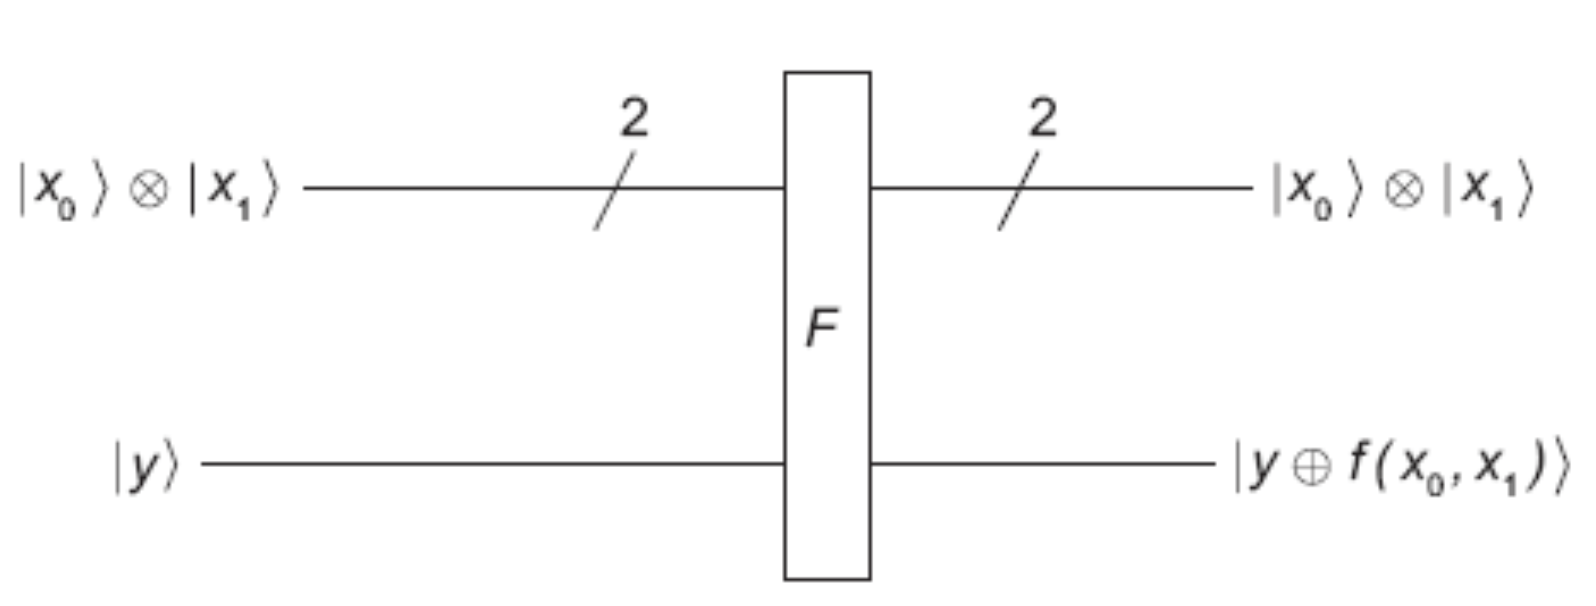
\includegraphics[width=0.8\linewidth]{Oracle}
	\caption{Оракул для функции $F$. Косые наклонные линии с числом $2$ означают обозначают параллельные входы и выходы.}
	\label{oracle}
\end{figure}

\begin{figure}[H]
	\centering
	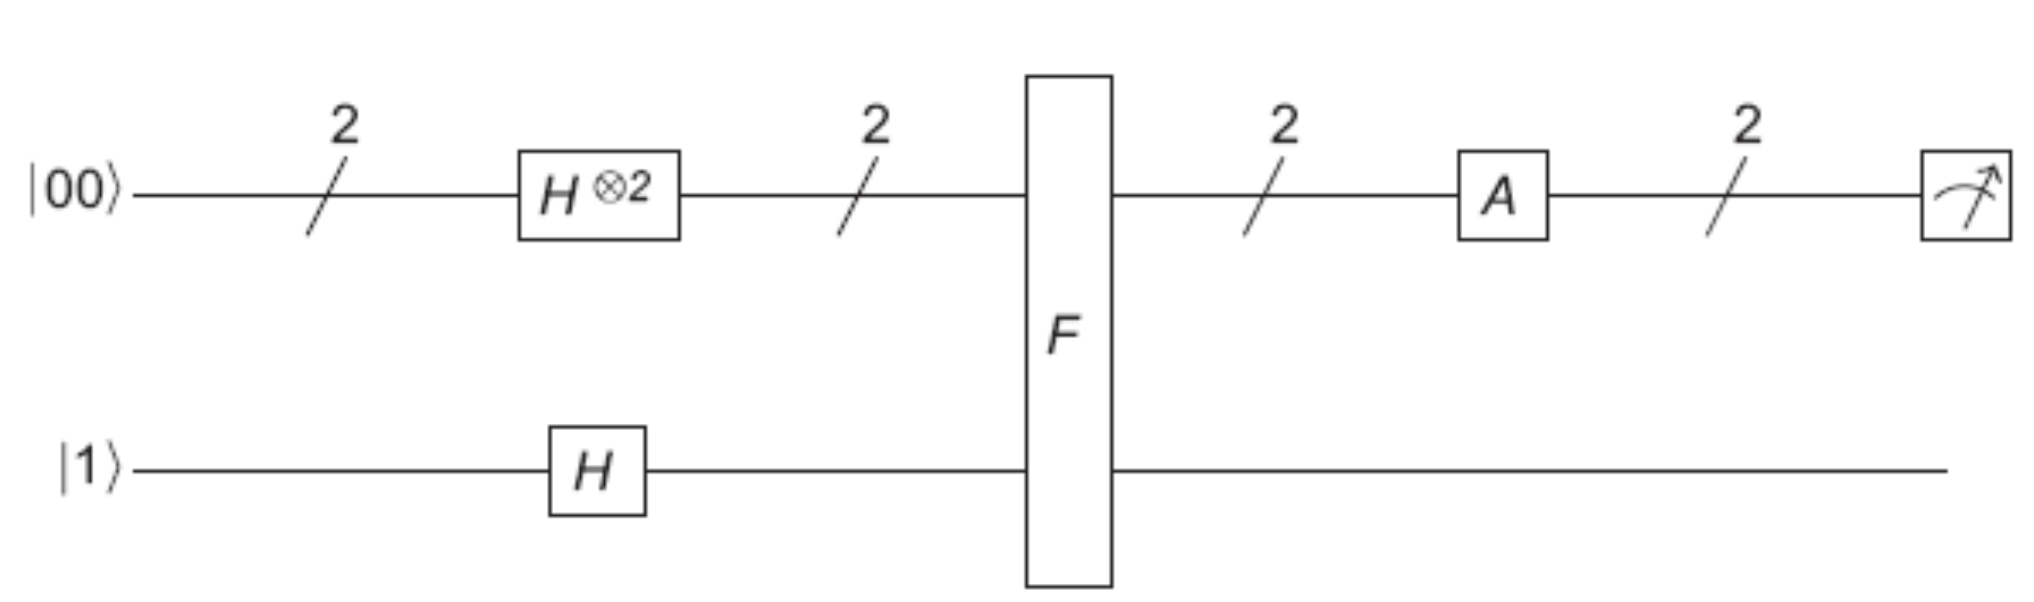
\includegraphics[width=0.8\linewidth]{Grover}
	\caption{Цепь алгоритма Гровера. Косые наклонные линии с числом $2$ означают обозначают параллельные входы и выходы.}
	\label{grover}
\end{figure}

После передачи данных через вентили Адамара два верхних кубита получают состояние:

\begin{equation}
	\frac{1}{2}\big(\ket{00} + \ket{01}+ \ket{10} + \ket{11}\big)
\end{equation}

Для нижнего же кубита:

\begin{equation}
	\frac{1}{\sqrt{2}}\big( \ket{0} - \ket{1}\big)
\end{equation}

После прохождения оракула происходит инвертирование $0$ и $1$ в третьем кубите в местоположение, которое нам нужно найти. Для нашего примера $F(10) = 1$:

\begin{align*}
	\frac{1}{2}\left[\ket{00} \otimes \frac{1}{\sqrt{2}}\big(\ket{0} - \ket{1} \big) + \ket{01} \otimes \frac{1}{\sqrt{2}}\big(\ket{0} - \ket{1} \big) + \ket{10} \otimes \frac{1}{\sqrt{2}}\big(\ket{1} - \ket{0} \big)\right. + \\
	\left.+ \ket{11} \otimes \frac{1}{\sqrt{2}}\big(\ket{0} - \ket{1} \big)\right]
\end{align*}

В компактной форме можно это переписать:

\begin{equation}
	\frac{1}{2}\big( \ket{00} + \ket{01} - \ket{10} + \ket{11}\big) \otimes \frac{1}{\sqrt{2}} \big(\ket{0} - \ket{1}\big)
\end{equation}

В результате мы получили два верхних кубита, ну спутанных с нижним, но амплитуда вероятности $\ket{10}$ поменяла знак, что и указывает на нужное местоположение.

Проделанного, однако, недостаточно: если на этом шаге измерить два верхних кубита, то мы равновероятно получим одну из четырех последовательностей, что нас не устраивает. Нам нужно теперь усилить амплитуда вероятности. Делается это путем переворачивания последовательности числе относительно их среднего: если число выше среднего, то оно перевернется и окажется ниже среднего и наоборот. В каждом случае расстояние до среднего очевидно сохраняется.

Для примера рассмотрим четыре числа: 1, 1, 1 и $-1$. Их среднее есть $1/2$. Посмотрим, что будет происходить при перевороте чисел. Первое, второе и третье числа выше среднего на $1/2$. Таким образом в результате переворота они превратятся в 0. Четвертое же число --- $-1$ --- меньше среднего и после переворота окажется равным 2.

В контексте нашей задачи мы имеем два верхних кубита в состоянии:

\begin{equation}
	\frac{1}{2}\ket{00} + \frac{1}{2}\ket{01} - \frac{1}{2}\ket{10} + \frac{1}{2}\ket{11}
	\label{sost}
\end{equation}

После переворота относительно среднего мы получим иные коэффициенты:

\begin{equation}
	0 \ket{00} + 0 \ket{01} + 1 \ket{10} + 0\ket{11} = \ket{10}
\end{equation}

Теперь после измерения мы гарантированно получим последовательность 10. Нужно только убедиться в существовании вентиля (или ортогональной матрицы), которая описывала бы переворот относительно среднего. Такая матрица существует и записывается как:

\begin{equation}
	A = \frac{1}{2}
	\begin{pmatrix}
		-1 & 1 & 1 & 1\\
		1 & -1 & 1 & 1\\
		1 & 1 & -1 & 1\\
		1 & 1 & 1 & -1
	\end{pmatrix}
\end{equation}

Если подставить ее действие на состояние \ref{sost}, то мы получим как раз нужное нам состояние. Таким образом в случае $n=2$ алгоритм Гровера позволяет гарантированно получить точный ответ после единственного обращения к функции $F$, что в 2.25 раза быстрее, чем в классическом случае.

Идея распространяется и на случай произвольного числа кубитов $n$. Алгоритм действия такой же: мы переворачиваем знак амплитуды вероятности, соответствующей искомой последовательности, после чего совершаем переворот относительно среднего и усиливаем амплитуду. Однако в этом случае вероятность будет меньше. Рассмотрим для примера восемь чисел (3 кубита), первые из которых равны 1, а последнее --- $-1$. Их среднее $6/8$, после переворота первые семь перейдут в $1/2$, а последнее --- в $10/4$. Видно, что вероятность нужного нам числа больше, чем других, но уже не равно 100\%. Нам нужно еще сильнее усилить амплитуду перед измерением.


Решением этой задачи может служить повторная передача кубитов через сеть. Таким образом нужная амплитуда усилится больше.

В общем случае задачу можно сформулировать так: из $m$ возможных последовательностей нужно найти нужную. В классическом случае нужно будет в худшем случае $m-1$ измерение, число вопросов растет как $O(m)$. В квантовом же случае, как было показано Гровером, ассимптотика меняется и сложность алгоритма составляет $O(\sqrt{m})$ для получения максимальной вероятности правильного ответа (нужно $\sqrt{m}$ раз <<прогнать>> задачу через цепь).

\section{Алгоритм Дойча}

Зададимся похожей задачей. Пусть теперь у нас есть одна переменная, которая может принимать значение либо 1, либо 0, а также 4 функции, которые устроены следующим образом:

\begin{align}
	f_0(0) = 0, \quad f_0(1) = 0\\
	f_1(0) = 0, \quad f_0(1) = 1\\
	f_2(0) = 1, \quad f_0(1) = 0\\
	f_3(0) = 1, \quad f_0(1) = 1
\end{align}

Функции, которые возвращают всегда одно и то же число ($f_0, f_3$), будем называть \textbf{константными}, функции, которые для половины значений возвращают 0, для половины --- 1 ($f_1, f_2$), будем называть \textbf{сбалансированными.}

Задача --- определить, какие функции являются сбалансированными, а какие --- константными за минимальное число вычислений.

С точки зрения классики для каждой функции, очевидно, нужно произвести два измерения. Рассмотрим задачу с квантовой точки зрения.

Сконструируем модель вентиля, представленную на рисунке \ref{DoiceF}.

\begin{figure}[H]
	\centering
	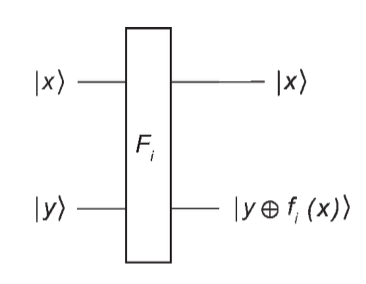
\includegraphics[width=0.6\linewidth]{DoiceF}
	\label{DoiceF}
	\caption{Оракул для функции $f_i$ в алгоритме Дойча}
\end{figure}

Согласно этой модели:

\begin{itemize}
	\item Если на вход подать $\ket{0} \otimes \ket{0}$, то она выведет $\ket{0} \otimes \ket{f_i(0)}$;
	
	\item Если на вход подать $\ket{0} \otimes \ket{1}$, то она выведет $\ket{0} \otimes \ket{f_i(0) \oplus 1}$;
	
	\item Если на вход подать $\ket{1} \otimes \ket{0}$, то она выведет $\ket{1} \otimes \ket{f_i(1)}$;
	
	\item Если на вход подать $\ket{1} \otimes \ket{1}$, то она выведет $\ket{0} \otimes \ket{f_i(1)}\oplus 1$.
\end{itemize}

Таким образом для каждого $i$ одна из $f_i(0)$, $f_i(0) \oplus 1$ равна 0, в то время как вторая равна 1 и аналогично для значения в 1. Таким образом четыре выхода всегда дают нам элементы стандартного базиса, т.е. матрица ортогональна, а значит модель действительно является вентилем.

Даже при том что мы вводим два бита информации и получаем два бита на выходе, информация, которую эти вентили дают для битов $\ket{0}$ и $\ket{1}$ такая же, как для функций, получающих 0 и 1. Верхний кубит --- то, что мы вводим, поэтому вывод не дает нам ничего нового. Выбирая же $\ket{0}$ или $\ket{1}$ для второго, то мы получаем второй выход, дающий нам тот же результат, что вернула функция для верхнего входного кета или противоположный, т.е. зная один мы знаем второй.

Если ограничиться только вводом $\ket{0}$ и $\ket{1}$, то мы придем к тому же ответу, что и прежде. Вентиль нужно использовать дважды, но Дойч показал, что если использовать суперпозиции этих векторов, то можно обойтись одним использованием вентиля.

Для доказательства этого факта рассмотрим цепь, представленную на рисунке \ref{Doice}. Кубиты $\ket{0} \otimes \ket{1}$ --- вход. Проходя через вентили Адамара, они перейдут в состояние:

\begin{equation}
	\frac{1}{\sqrt{2}}\big(\ket{0} + \ket{1}\big) \otimes \frac{1}{\sqrt{2}} \big(\ket{0} - \ket{1}\big) = \frac{1}{2} \big(\ket{00} - \ket{01} + \ket{10} - \ket{11}\big)
\end{equation}

\begin{figure}[H]
	\centering
	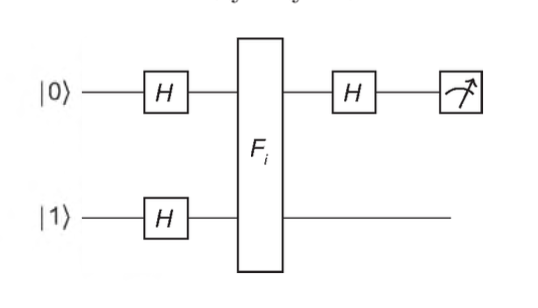
\includegraphics[width=0.8\linewidth]{Doice}
	\label{Doice}
	\caption{Цепь алгоритма Дойча}
\end{figure}

Затем после прохождения вентиля $F_i$:

\begin{equation}
	\frac{1}{2}\big(\ket{0} \otimes \ket{f_i(0)} - \ket{0} \otimes \ket{f_i(0) \oplus 1} + \ket{1} \otimes \ket{f_i(1)} - \ket{1} \otimes \ket{f_i(1) \oplus 1} \big)
\end{equation}

Упрощая:

\begin{equation}
	\frac{1}{2}\bigg(\ket{0} \otimes \big(\ket{f_i(0)} - \ket{f_i(0) \oplus 1}\big) + \ket{1} \big(\ket{f_i(1)} - \ket{f_i(1)} \oplus 1\big) \bigg)
\end{equation}

Заметим, что верно выражение:

\begin{equation}
	\ket{f_i(0)} - \ket{f_i(0) \oplus 1} = (-1)^{f_i(0)} \big(\ket{0} - \ket{1}\big)
\end{equation}

А также:

\begin{equation}
	\ket{f_i(1)} - \ket{f_i(1) \oplus 1} = (-1)^{f_i(1)} \big(\ket{0} - \ket{1}\big)
\end{equation}

Тогда полученное выражение переписывается:

\begin{equation}
	\frac{1}{2}\bigg(\ket{0} \otimes \big((-1)^{f_i(0)}(\ket{0} - \ket{1})\big) + \ket{1} \otimes \big((-1)^{f_i(1)}(\ket{0} - \ket{1})\big)\bigg)
\end{equation}

Упрощая, получим итоговое выражение:

\begin{equation}
	\frac{1}{\sqrt{2}} \big((-1)^{f_i(0)}\ket{0} + (-1)^{f_i(1)}\ket{1}\big) \otimes \frac{1}{\sqrt{2}} \big(\ket{0} - \ket{1}\big)
\end{equation}

Таким образом два кубита не спутаны и верхний кубит имеет состояние:

\begin{equation}
	\frac{1}{\sqrt{2}} \big((-1)^{f_i(0)}\ket{0} + (-1)^{f_i(1)}\ket{1}\big)
\end{equation}

Исследуем это состояние для каждой из возможных $f_i$:

\begin{itemize}
	\item Для $f_0$ мы имеем $f_0(0) = f_0(1) = 0$, то есть кубит имеет состояние $(1/\sqrt{2}) (\ket{0} + \ket{1})$.
	
	\item Для $f_1$ мы имеем $f_1(0) = 0$ и $f_1(1) = 1$, то есть кубит имеет состояние $(1/\sqrt{2}) (\ket{0} - \ket{1})$.
	
	\item Для $f_2$ мы имеем $f_2(0) = 1$ и $f_2(1) = 0$, то есть кубит имеет состояние $-(1/\sqrt{2}) (\ket{0} - \ket{1})$.
	
	\item Для $f_3$ мы имеем $f_3(0) = f_3(1) = 1$, то есть кубит имеет состояние $-(1/\sqrt{2}) (\ket{0} + \ket{1})$.
\end{itemize}

Следующий шаг это еще одна передача в вентиль Адамара. В результате мы получим:

\begin{itemize}
	\item если $i = 0$, то кубит имеет состояние $\ket{0}$;
	
	\item если $i = 1$, то кубит имеет состояние $\ket{1}$;
	
	\item если $i = 2$, то кубит имеет состояние $-\ket{1}$;
	
	\item если $i = 3$, то кубит имеет состояние $-\ket{0}$.
\end{itemize}

Теперь если мы измерим кубит в стандартном базисе, то мы получим 0, если $i = 0, 3$ и 1, если $i=1, 2$, т.е. мы гарантированы отделяем константные функции от сбалансированных. Таким образом, мы можем обойтись одним обращением к оракулу.

\section{Алгоритм Дойча-Йожи}

Рассмотрим алгоритм Дойча, но теперь с функциями не одной, а $n$ переменных. Каждая из них как и прежде приобретает значение 0 или 1. Концепция константной функции не меняется, а сбалансированная функция должна давать 0 для половины комбинаций выходов, а для второй половины должна возвращать 1. Задача остается той же, нужно понять, является ли случайная функция сбалансированной или константной.

Для примера рассмотрим случай $n=3$. Тогда у нас есть $2^3 = 8$ различных входных комбинаций.

Рассматривая задачу с классической точки зрения можно показать, что в общем случае нужно в худшем случа задать $2^{n-1} + 1$ вопрос, т.е. сложность экспоненциальная.

Перейдем к квантовому описанию Для каждой функции $f_i$ $n$ булевых переменных сконструируем вентиль $F$, представленный на рисунке \ref{Doice-JozheF}. Здесь косые наклонные линии с числом $n$ означают обозначают параллельные входы и выходы.

\begin{figure}[H]
	\centering
	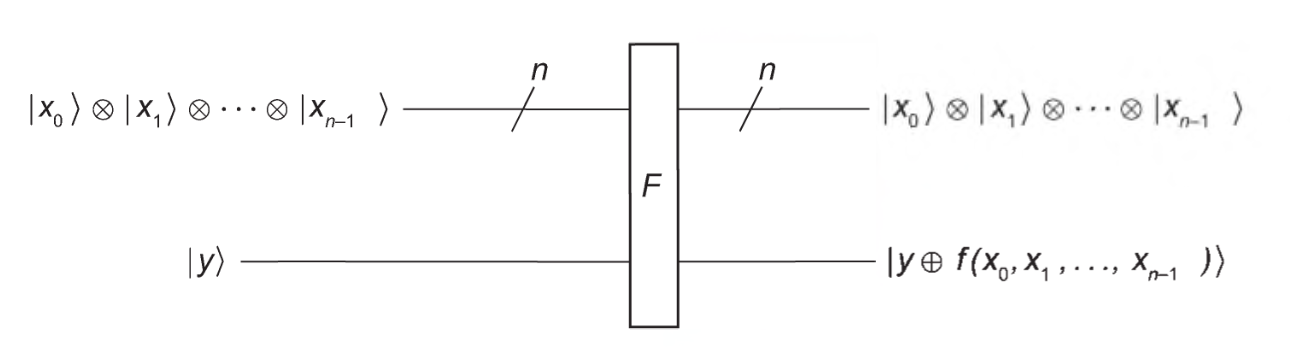
\includegraphics[width=0.8\linewidth]{Doice-JozheF}
	\label{Doice-JozheF}
	\caption{Оракул для функции $f_i$ в алгоритме Дойча-Йожи}
\end{figure}

Эта цепь сообщает нам, что происходит, когда каждый из $\ket{x_i}$ представлен как $\ket{0}$ или $\ket{1}$. На входе имеем $n+1$ кетов, представимых в виде:

\begin{equation}
	\ket{x_0} \otimes \ket{x_1} \otimes ...  \otimes \ket{x_{n-1}}
\end{equation}

а также $\ket{y}$, где первые $n$ кетов соответствуют входным переменным. На выходе же мы видим $n+1$ кетов, первые $n$ из которых в точности совпадают со входными кетами, в то время как последний выходной будет равне $\ket{f(x_0, x_1, ..., x_{n-1})}$, если $y=0$ и кет с другим \textbf{булевым} значением, если $y=1$.

Квантовая цепь для алгоритма выглядит так, как представлено на рисунке \ref{Doice-Jozhe}. Для упрощения задачи придется рассматривать $n=2$ с оговоркой, что большие $n$ работают так же.

\begin{figure}[H]
	\centering
	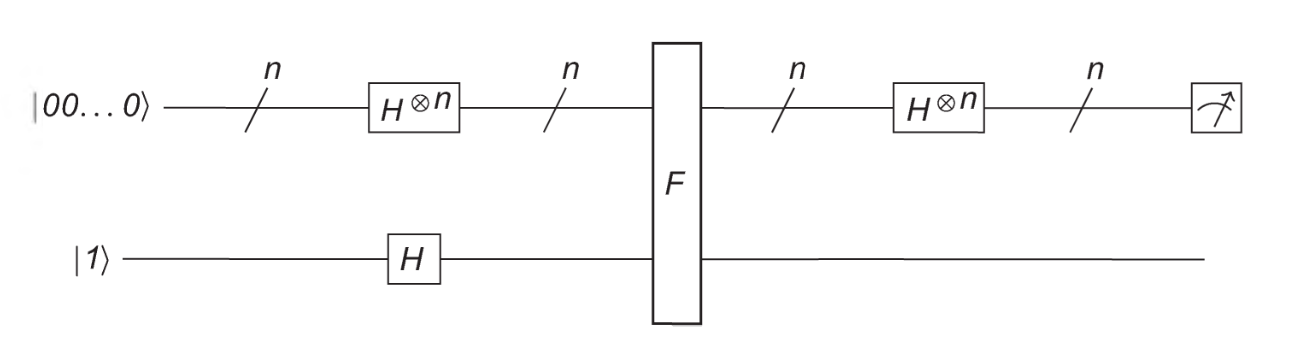
\includegraphics[width=0.8\linewidth]{Doice-Jozhe}
	\label{Doice-Jozhe}
	\caption{Цепь алгоритма Дойча-Йожи}
\end{figure}

Первым этапом происходит передача кубитов через вентили Адамара. Все верхние $n$ входов равны $\ket{0}$, т.е. в нашем случае это $\ket{00}$. После применения вентиля состояние:

\begin{equation}
	\frac{1}{2}\big(\ket{00} + \ket{01} + \ket{10} + \ket{11}\big)
\end{equation}

Нижний же выход это просто $\ket{1}$. После прохождения кубита через вентиль будет состояние:

\begin{equation}
	\frac{1}{\sqrt{2}}\big(\ket{0} - \ket{1}\big)
\end{equation}

Таким образом общее состояние:

\begin{equation}
	\frac{1}{2} \big(\ket{00} + \ket{01} + \ket{10} + \ket{11}\big) \otimes \frac{1}{\sqrt{2}}\big(\ket{0} - \ket{1}\big)
\end{equation}

Мы можем переписать это выражение как:

\begin{equation}
	\frac{1}{2\sqrt{2}}\bigg(\ket{00} \otimes \big(\ket{0} - \ket{1}\big) + \ket{01} \otimes \big(\ket{0} - \ket{1}\big) + \ket{10} \otimes \big(\ket{0} - \ket{1}\big) + \ket{11} \otimes \big(\ket{0} - \ket{1}\big) \bigg)
\end{equation}

После перехода через вентиль $F$ получится состояние:

\begin{align*}
	\frac{1}{2\sqrt{2}} \ket{00} \otimes \big(\ket{f(0, 0)} - \ket{f(0, 0) \oplus 1}\big) + \frac{1}{2\sqrt{2}} \ket{01} \otimes \big(\ket{f(0, 1)} - \ket{f(0, 1) \oplus 1}\big) + \\
	+ \frac{1}{2\sqrt{2}} \ket{10} \otimes \big(\ket{f(1, 0)} - \ket{f(1, 0) \oplus 1}\big) + \frac{1}{2\sqrt{2}} \ket{11} \otimes \big(\ket{f(1, 1)} - \ket{f(1, 1) \oplus 1}\big)
\end{align*}

Далее, если какое-то $a$ может принимать только значения $0$ или $1$, тогда выполняется равенство:

\begin{equation}
	\ket{a} - \ket{a\oplus 1} = (-1)^a (\ket{0} - \ket{1})
\end{equation}

С учетом этого факта:

\begin{align}
	(-1)^{f(0, 0)} \frac{1}{2} \ket{00} \otimes \frac{1}{\sqrt{2}} \big(\ket{0} - \ket{1}\big) + (-1)^{f(0, 1)} \frac{1}{2} \ket{01} \otimes \frac{1}{\sqrt{2}} \big(\ket{0} - \ket{1}\big) + \\
	+ (-1)^{f(1, 0)} \frac{1}{2} \ket{10} \otimes \frac{1}{\sqrt{2}} \big(\ket{0} - \ket{1}\big) + (-1)^{f(1, 1)} \frac{1}{2} \ket{11} \otimes \frac{1}{\sqrt{2}} \big(\ket{0} - \ket{1}\big)
\end{align}

Отсюда видно, что нижний кубит с верхними не запутан. Рассмотрим теперь просто два верхних кубита. Они находятся в состоянии:

\begin{equation}
	\frac{1}{2}\bigg((-1)^{f(0, 0)} \ket{00} + (-1)^{f(0, 1)}\ket{01} + (-1)^{f(1, 0)}\ket{10} + (-1)^{f(1, 1)}\ket{11}\bigg)
\end{equation}

Такое доказательство (идейно) будет верным для любого $n$. 

Теперь нужно преобразовать состояние в вектор столбец с последующем умножением на соответствующее кронекеровское произведение матрицы Адамара. Нам, однако, не требуется вычислять все элементы, нам хватит только верхнего элемента, который будет получаться умножением бра, соответствующим верхней строке матрицы, на кет, заданный вектором-столбцом. Опуская вычисления:

\begin{equation}
	\frac{1}{4}\bigg((-1)^{f(0, 0)} + (-1)^{f(0, 1)} + (-1)^{f(1, 0)} + (-1)^{f(1, 1)}\bigg)
\end{equation}

Это амплитуда вероятности кета $\ket{00}$. Вычислим эту амплитуду для разных функций:

\begin{itemize}
	\item Если $f$ константная и всегда возвращает 0, то амплитуда вероятности равна 1;
	
	\item Если $f$ константная и всегда возвращает 1, то амплитуда вероятности равна -1;
	
	\item Для сбалансированных функций амплитуда вероятности равна 0.  
\end{itemize}

Измерив верхние кубиты, мы получим одно из значений: 00, 01, 10 или 11. Подумаем, когда мы получим 00. Если функция константная, то мы получим 1. Если сбалансированная, то 0. То есть если мы получаем 00, то можно утверждать, что функция константная. В случае любого другого отличного от 00 результата мы можем утверждать, что функция была сбалансированной.

Аналогичные размышления верны и для любого $n$. Непосредственно перед измерением кубитов амплитуда вероятности для $\ket{0...0}$ равна:

\begin{equation}
	\frac{1}{2^n}\bigg((-1)^{f(0, 0, ..., 0)} + (-1)^{f(0, 0, ..., 1)} + ... + (-1)^{f(1, 1, ..., 1)}\bigg)
\end{equation}

Как и для $n=2$ в результате будет $\pm1$, если $f$ --- константная и 0, если $f$ сбалансированная. Если все измерения дают 0, то функция константная, в противном случае --- сбалансированная.

Таким образом нам нужно задавать оракулу \textbf{всего один вопрос}, в то время как в классическом алгоритме сложность была экспоненциальна. Очевидно значительное ускорение выполнения задачи.





\end{document}